\wcht{Coupon collector problem}: niech $X$ oznacza zmienną losową, jak długo należy zbierać kupony, aby zebrać każdy z nich co najmniej raz.
%http://en.wikipedia.org/wiki/Coupon_collector%27s_problem_%28generating_function_approach%29
\wcht{German tank problem}: jeśli dostrzeżono $k$ czołgów o najwyższym numrze $m$, to wszystkich jest w przybliżeniu $m + m/k-1$.
%Bayesian analysis: $N \approx \mu \pm \sigma$, gdzie $\mu = (m-1)(1+1/(k-2))$, zaś $\sigma^2 = (k-1)(m-1)(m-k+1)/(k-3)(k-2)^2$.
\[
	\ex \iks = n H_n \spk
	\war \iks = \sum_{k=1}^n (n/k)^2 - nH_n < \frac{(\pi n)^2}{6} \spk
	d = \frac{r}{\sqrt{2}}
\]
$P(A_i)$: a priori (przed), $P(A_i \mid B)$: a posteriori (po).

\wcht{Model urnowy}: urna zawiera $x$ czarnych i $y$ czerwonych kul, wylosowaną zastępuje $a$ losowanych i $b$ drugiego koloru (losowanie bez końca).
\wcht{Polya}: $b = 0$ i $a > 0$ \emph{(contagious diseases}, jeden wypadek pociąga następne).
P-stwo, że z $n = n_1 + n_2$ losowań pierwsze $n_1$ będzie czarne, pozostałe czerwone, daje {lewy wzór}.
P-stwo, że $n_1$ czarnych i $n_2$ czerwonych rozłoży się dowolnie zadane jest {prawym wzorem}.
Model Ehrenfesta wymiany ciepła: $k$ cząsteczek w dwóch pojemnikach, losowo wybrana zostaje przeniesiona do drugiego, jaki jest ich rozkład po $n$ losowaniach? $(a,b) = (-1,1)$.
\[
	{p_1} = \frac{\left[\prod_{k=1}^{n_1}(x+(k-1)a)\right]\left[\prod_{k=1}^{n_2}(y+(k-1)a)\right] }{\left[\prod_{k=1}^{n}(x+y+(k-1)a)\right]} \spk
	{p_2} = \dwum{-x/a}{n_1} \dwum{-y/a}{n_2} \left/\dwum{-(x+y)/a}{n}\right.
\]

\wcht{{Momenty}}: $\mu_n = \ex [\iks^n]$.
\wcht{{Funkcja tworząca p-stwa}}: $G_\iks(z) = \sum_{k \ge 0} P(\iks = k) z^k = \ex[\exp \iks]$, dla zmiennych niezależnych: $G_{\iks + \igr}= G_\iks G_\igr$. Fakt: $\ex \iks = G_\iks'(1)$ i $\war \iks = G_\iks''(1) + G_\iks'(1)-G_\iks'(1)^2$.
Jeśli $G(z)$ jest ftp dla $X$, to {lewa tożsamość}.
\wcht{{Półniezmienniki}} (Thiele, \datum{1903}) są ważniejsze od momentów.
$\kappa_1$ to średnia, $\kappa_2$ to wariancja, dalej tak, jak {po prawej}.
\end{parnumbers}

> Kiedy byłem młody wydawało mi się że pieniądze są najważniejsze. Teraz jestem już tego pewien Oskar Wilde :)

## Teoria mnogości
* Normal function (ordinals)

## Teoria liczb
* http://en.wikipedia.org/wiki/List_of_number_theory_topics
* http://en.wikipedia.org/wiki/List_of_recreational_number_theory_topics
* Wzór Möbiusa mówi, że $$E_p(x) = \prod_{(p,n)=1}(1-x^n)^{-\mu(n)/n}$$

## Hnnng
* bhp dla szeregów :D zadanie dla lakoffa i nuneza: przy użyciu basic metaphor o infinity skonstruować szereg najwolniej rozbieżny.
* Twierdzenie Pompeiu
* Fano plane.
* Krzywe eliptyczne, automorfizm Frobeniusa
* Funkcje tworzące dla p-stw

## Algebra
* Zasadnicze Twierdzenie Algebry

## Geometria
* http://en.wikipedia.org/wiki/List_of_circle_topics 
* http://en.wikipedia.org/wiki/List_of_trigonometry_topics
* http://en.wikipedia.org/wiki/Outline_of_trigonometry
* http://en.wikipedia.org/wiki/List_of_surfaces
* http://en.wikipedia.org/wiki/List_of_trigonometric_identities
* http://en.wikipedia.org/wiki/List_of_triangle_topics
* http://en.wikipedia.org/wiki/List_of_geometric_topology_topics
* http://en.wikipedia.org/wiki/Lagrange%27s_trigonometric_identities#Lagrange.27s_trigonometric_identities

* http://en.wikipedia.org/wiki/List_of_differential_geometry_topics
* http://en.wikipedia.org/wiki/Monge%27s_theorem
* Stewart, SteinerLehmus, Desargues
* http://en.wikipedia.org/wiki/List_of_geometry_topics
* http://en.wikipedia.org/wiki/Outline_of_geometry

## Analiza 
* Conway base 13 function, Fredholmsche Integralgleichung 2. Art: $y(t) + \int_0^1 K(t,s) y(s) \, \textrm{d}s = g(t)$, Variationsrechnung: $F[y] = \int_0^1 f(t, y(t), y'(t))\, \textrm{d} t$ (minimalizacja)
* Funkcja Airy'ego

## Teoria mnogości
* Normal function (ordinals)

## Teoria liczb
* http://en.wikipedia.org/wiki/List_of_number_theory_topics
* http://en.wikipedia.org/wiki/List_of_recreational_number_theory_topics
* Wzór Möbiusa mówi, że $$E_p(x) = \prod_{(p,n)=1}(1-x^n)^{-\mu(n)/n}$$

## Hnnng
* bhp dla szeregów :D zadanie dla lakoffa i nuneza: przy użyciu basic metaphor o infinity skonstruować szereg najwolniej rozbieżny.
* Twierdzenie Pompeiu
* Fano plane.
* Krzywe eliptyczne, automorfizm Frobeniusa
* Funkcje tworzące dla p-stw

## Algebra
* Zasadnicze Twierdzenie Algebry

## Geometria
* http://en.wikipedia.org/wiki/List_of_circle_topics 
* http://en.wikipedia.org/wiki/List_of_trigonometry_topics
* http://en.wikipedia.org/wiki/Outline_of_trigonometry
* http://en.wikipedia.org/wiki/List_of_surfaces
* http://en.wikipedia.org/wiki/List_of_trigonometric_identities
* http://en.wikipedia.org/wiki/List_of_triangle_topics
* http://en.wikipedia.org/wiki/List_of_geometric_topology_topics
* http://en.wikipedia.org/wiki/Lagrange%27s_trigonometric_identities#Lagrange.27s_trigonometric_identities

* http://en.wikipedia.org/wiki/List_of_differential_geometry_topics
* http://en.wikipedia.org/wiki/Monge%27s_theorem
* Stewart, SteinerLehmus, Desargues
* http://en.wikipedia.org/wiki/List_of_geometry_topics
* http://en.wikipedia.org/wiki/Outline_of_geometry







Iloczyn skalarny: kanoniczny: $\sum x_i y_i$, inny: $\int_0^1 fg$.
Iloczyn mieszany: $\langle A \times B, C \rangle$, $\det(ABC)$.
\wcht{Iloczyn wektorowy} pary $U = (x_1, y_1, z_1)$ i $W = (x_2, y_2, z_2)$ jest dwuliniowy, antysymetryczny i prostopadły do argumentów.
\hfill $\langle AX, Y \rangle = \langle X, A^TY\rangle$.
\[
	U \times W = \left(\begin{vmatrix} y_1 & y_2 \\z_1 & z_2\end{vmatrix}, - \begin{vmatrix} x_1 & x_2 \\z_1 & z_2\end{vmatrix}, \begin{vmatrix} x_1 & x_2 \\y_1 & y_2\end{vmatrix}\right)^T\spk
	\|U\times W\| = \|U\| \cdot \|W\| \cdot \sin \angle (U,W)
\]


afiniczne: liniowe złożone z translacją.
\wcht{Wartość, wektor własny}: $Av = \lambda v$, \wcht{ślad}: suma wyrazów na przekątnej, \wcht{wielomian charakterystyczny}: $\det(A-t I)$, \wcht{tw. Cayleya-Hamiltona}: każdy liniowy operator zeruje swój wielomian charakterystyczny.
\wcht{Tw. spektralne}: każda macierz symetryczna rozkłada się jako $Q \Lambda Q^T$, gdzie $\Lambda$ jest rzeczywistą macierzą diagonalną, zaś $Q$ jest ortogonalna ($Q^{-1} = Q^T$)


\wcht{(Macierzowe) grupy klasyczne}.
GL: odwracalne.
O: $AA^T = I$.
U: $AA^* = I$.
S: $\det A = 1$.
GL i O są z $M_{n \times n}(\R)$, U z $M_{n \times n}(\C)$

Diagonalizowalność: $A = S \Lambda S^{-1}$, $S$ to macierz wektorów własnych, $\Lambda$ to $\text{diag}(\lambda_1, \dots, \lambda_n)$.
Zawsze możliwa, gdy jest $n$ lnz wektorów własnych ($AM = GM$), wtedy $A^k=S \Lambda^k S^{-1}$.
Krotność geometryczna: wymiar jądra $A - \lambda I$, algebraiczna: krotność pierwiastka wielomianu charakterystycznego.
Dwie diagonalizujące się macierze mają tę samą macierz przejścia $\Leftrightarrow$ komutują.
%Wartości własne macierzy symetrycznej są rzeczywiste.
\wcht{Macierz Jordana}: $J$.
Nad algebraicznie domkniętym ciałem istnieje rozkład $A = P J P^{-1}$.
$J = \text{diag}(J_1, J_2, \dots, J_k)$.
Ilość kolumn $J_i$ odpowiada krotności (geometrycznej) wartości własnej.
$J_i$ ma $\lambda_i$ na przekątnej i jedynki nad nią.

\wcht{Mazur, Ulam}: surjektywna izometria między przestrzeniami unormowanymi nad $\mathbb R$ jest afiniczna.
\wcht{Beckman, Quarles}: odwzorowanie $\mathbb R^n \to \mathbb R^n$ ($n > 1$) przekształcające odcinki jednostkowe na jednostkowe jest izometrią.


Macierz \wcht{nilpotentna}: $N \neq 0$, ale $N^k = 0$; wielomian charakterystyczny to $\lambda^n$;  $\text{tr }(N^p) = 0$ dla $p \ge 1$.
Jeśli $N$ jest nilpotentna, to $\det (I+N) = 1$, jeśli dla każdego $t$ jest  $\det(I+tA) = 1$, to $A$ jest nilpotentna.
Osobliwa jest iloczynem nilpotentnych, tylko zerowa się diagonalizuje.
$I+N$ jest odwracalna: $(I+N)^{-1} = I - N + N^2 - N^3 + \dots$

\wcht{Funkcjonał}: liniowe $f: V \to \mathbb K$, tworzą przestrzeń dualną.
Jeśli $\dim V = n$, to $\dim V^* = n$, ta druga ma bazę: $e^i(e_j) = [i = j]$.
Jeśli $f:V\to W$ jest liniowe, to \wcht{dualne}, $f:W^* \to V^*$ zadane przez $f^*(\alpha) = \alpha \circ f$, też.
Fakt: $(h \circ f)^* = f^* \circ h^*$.
Jeśli $\dim V < \infty$, to istnieje kanoniczny ?-morfizm $\varepsilon: V \to V^{**}$: $\varepsilon(x) = \varepsilon_x$, $\varepsilon_x(f) = f(x)$, gdzie $x \in V$, $f \in V^*$, $\varepsilon_x \in V^{**}$.
$V$ (dowolnego wymiaru) jest \wcht{refleksywna}, jeśli $\varepsilon$ jest izomorfizmem. 
Domknięte jądro $\Leftrightarrow$ ciągła forma.

\wcht{Forma dwuliniowa}: dwuliniowe $f\colon V \times V \to \mathbb K$.
\wcht{Symetryczna}: $f(x,y) = f(y,x)$, \wcht{antysymetryczna}: $f(x,y) = - f(y,x)$.
Zmiana bazy: $F' = A^T \cdot F \cdot A$.
Rozkład: $F = (F+ F^T)/2 + (F-F^T)/2$.
$f(x, y) = X^T \cdot F \cdot Y$, gdzie $F = (f_{ij}) = (f(e_i, e_j))$ jest macierzą formy (tylko skończenie wymiarowe $V$).
Fakt: jeśli $\text{char } \K \neq 2$, to $L_2(V, \K) = L_2^+(V, \K) \oplus L_2^-(V, \K)$ (suma prosta symetrycznych i antysymetrycznych).



{
\begin{multicols}{2}
\begin{enumx} 
\item \farba{$(ax)^2 + (by)^2 + (cz)^2 = 1$ \hfill {\footnotesize {\bf} elipsoida}}
\item \farba{$(ax)^2 + (by)^2 - (cz)^2 = 1$ \hfill {\footnotesize {\bf} hiperboloida 1-powłokowa}}
\item \farba{$(ax)^2 - (by)^2 - (cz)^2 = 1$ \hfill {\footnotesize {\bf} hiperboloida 2-powłokowa}}
\item \farba{$(ax)^2 + (by)^2 - 2z = 0$ \hfill {\footnotesize {\bf} paraboloida eliptyczna}}
\item \farba{$(ax)^2 - (by)^2 - 2z = 0$ \hfill {\footnotesize {\bf} paraboloida hiperboliczna}}
\item \farbaa{$(ax)^2 + (by)^2 - (cz)^2 = 0$ \hfill {\footnotesize {\bf} stożek eliptyczny}}
\item \farbaa{$(ax)^2 + (by)^2 = 1$ \hfill {\footnotesize {\bf} walec eliptyczny}}
\item \farbaa{$(ax)^2 - (by)^2 = 1$ \hfill {\footnotesize {\bf} walec hiperboliczny}}
\item \farbaa{$(ax)^2 - 2y = 0$ \hfill {\footnotesize {\bf} walec paraboliczny}}
\item $(ax)^2 + (by)^2 + (cz)^2 = 0$ \hfill {\footnotesize {\bf} punkt}
\item $(ax)^2 + (by)^2 = 0$ \hfill {\footnotesize {\bf} prosta}
\item $(ax)^2 - (by)^2= 0$ \hfill {\footnotesize {\bf} dwie płaszczyzny przecinające się}
\item $(ax)^2 = 1$ \hfill {\footnotesize{\bf} dwie płaszczyzny równoległe}
\item $(ax)^2 = 0$ \hfill {\footnotesize{\bf} jedna płaszczyzna}
\end{enumx}
\end{multicols}
\begin{center}
\fbox{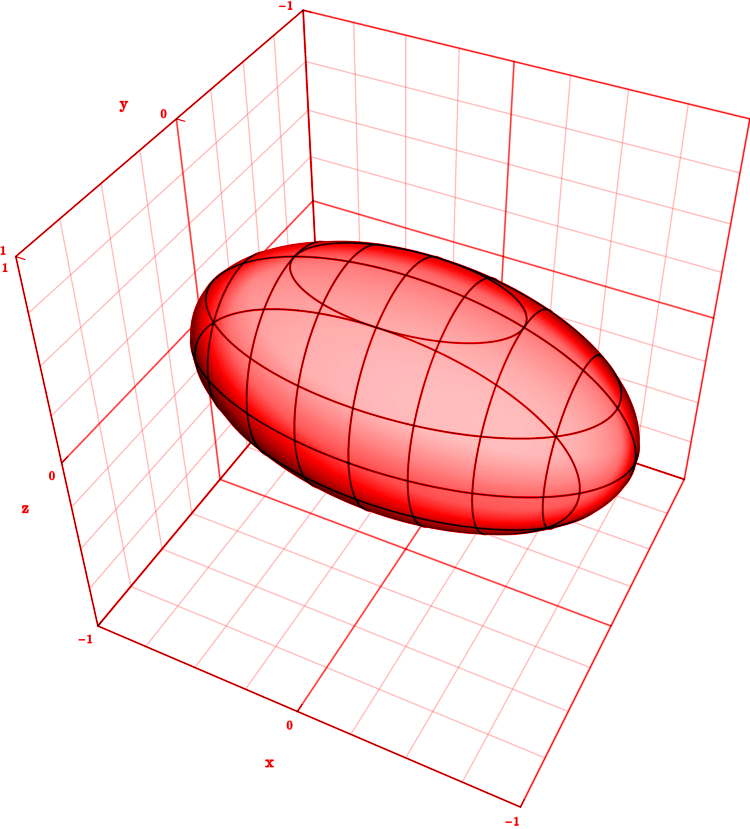
\includegraphics[height=0.183\columnwidth]{src/q1.png}}
\fbox{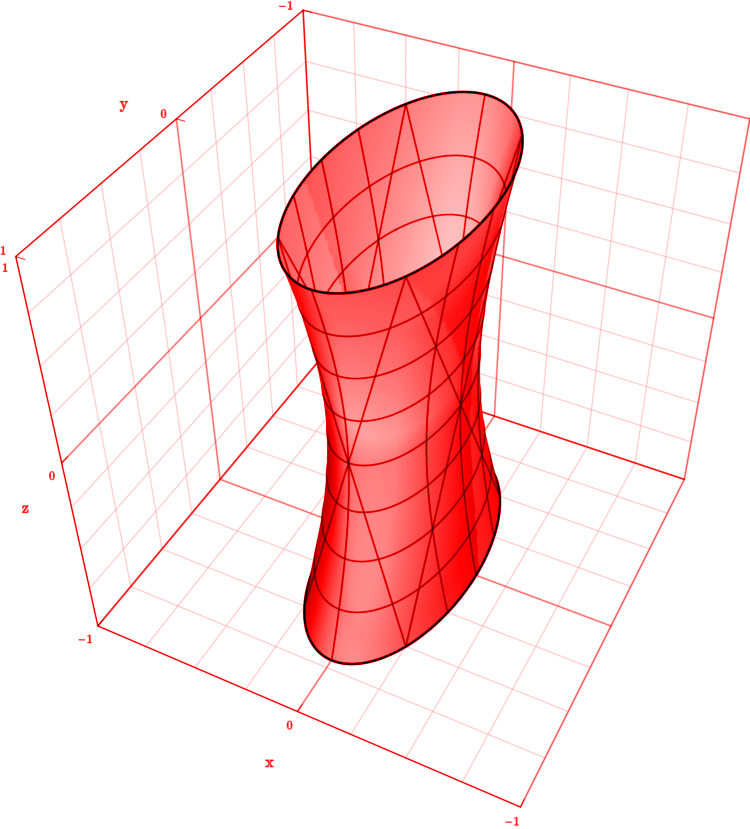
\includegraphics[height=0.183\columnwidth]{src/q2.png}}
\fbox{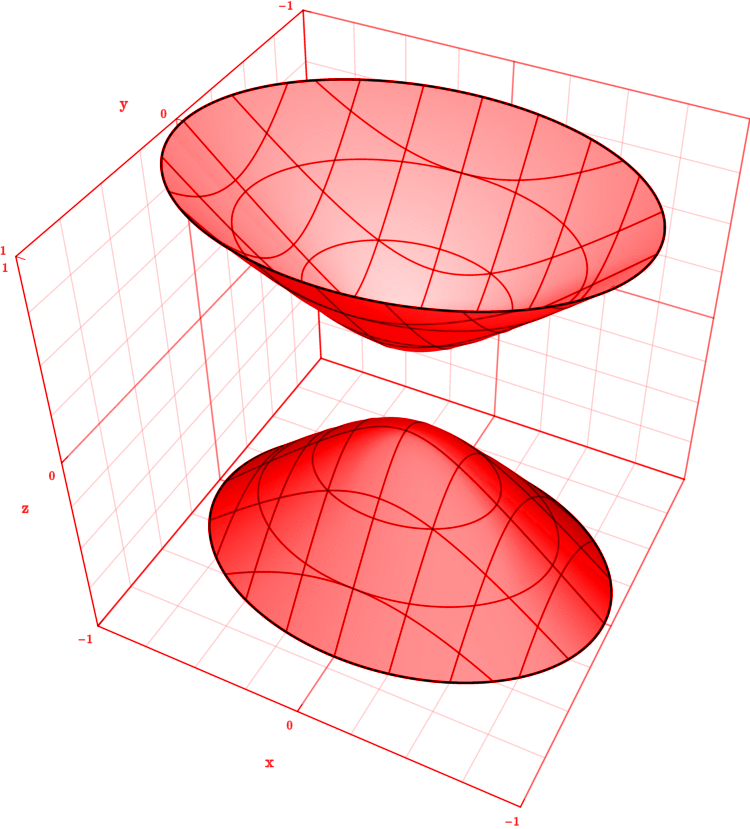
\includegraphics[height=0.183\columnwidth]{src/q3.png}}
\fbox{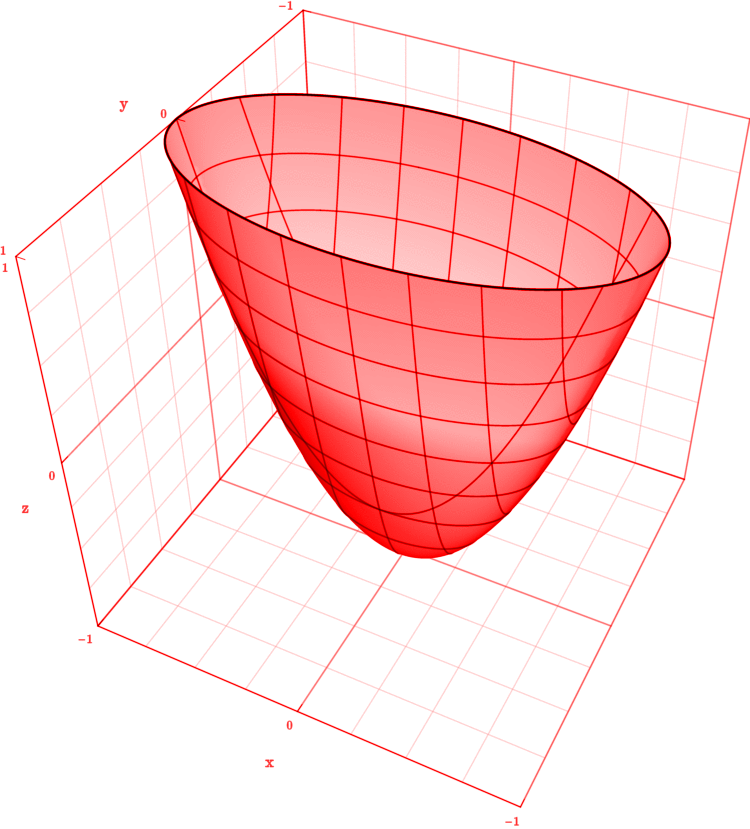
\includegraphics[height=0.183\columnwidth]{src/q4.png}}
\fbox{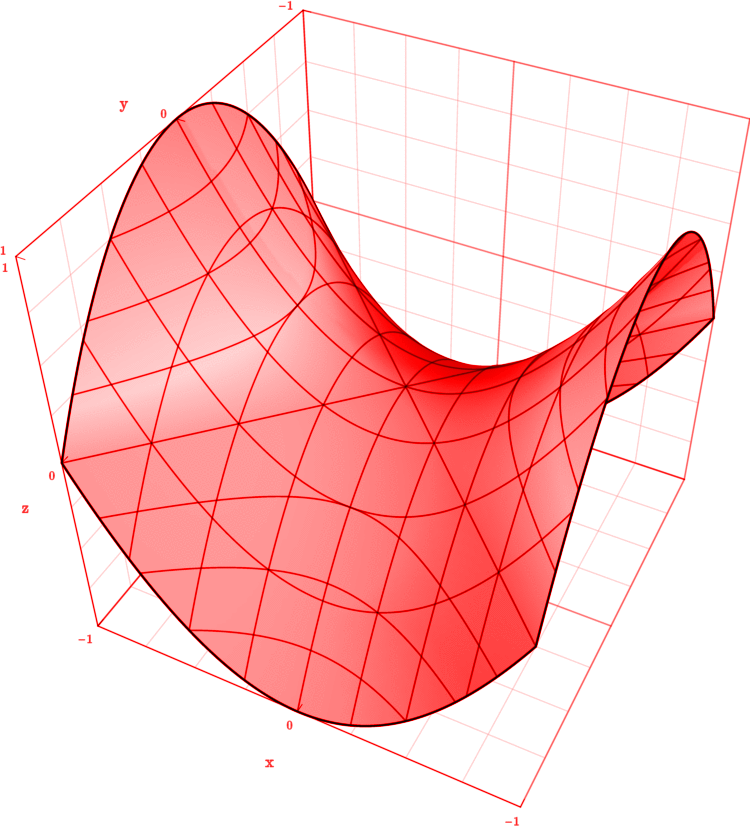
\includegraphics[height=0.183\columnwidth]{src/q5.png}}
\fbox{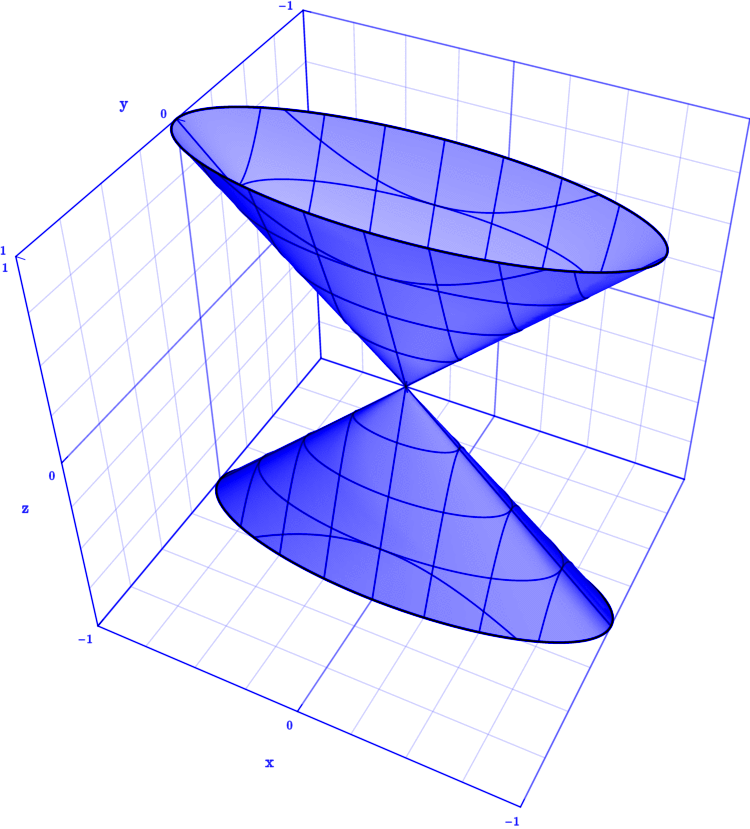
\includegraphics[height=0.183\columnwidth]{src/q6.png}}
\fbox{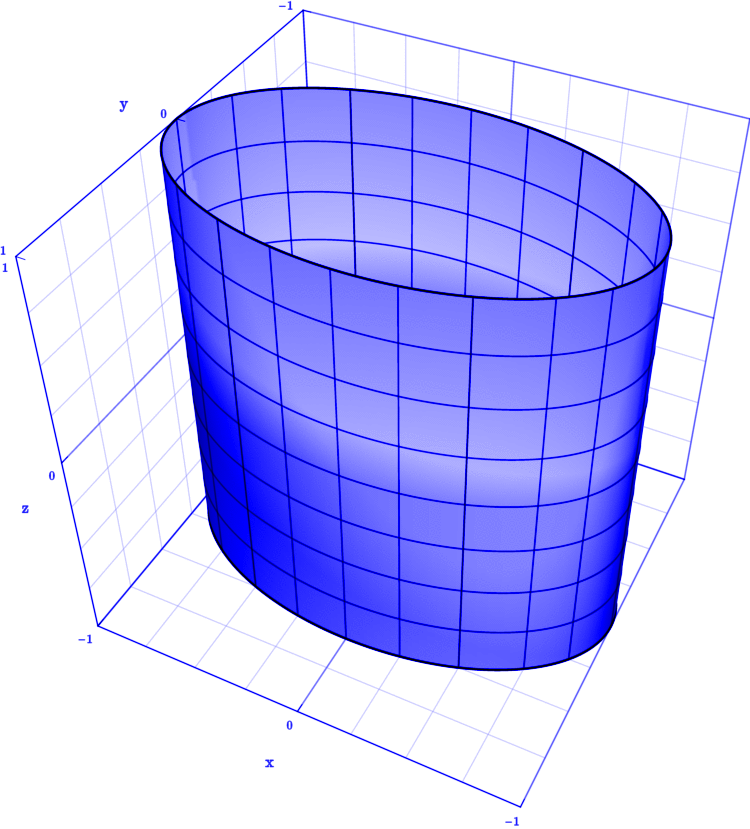
\includegraphics[height=0.183\columnwidth]{src/q7.png}}
\fbox{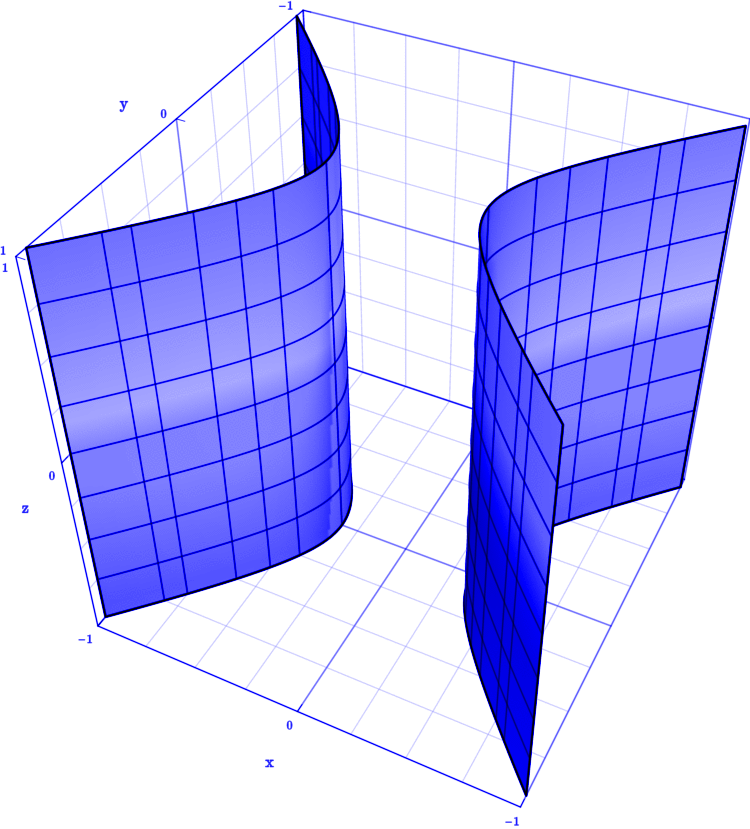
\includegraphics[height=0.183\columnwidth]{src/q8.png}}
\fbox{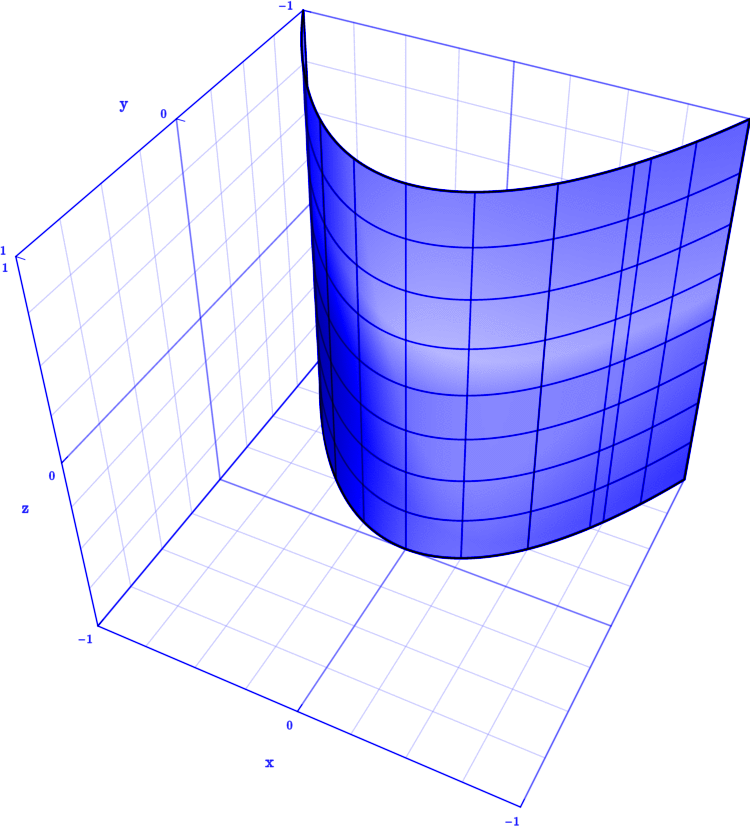
\includegraphics[height=0.183\columnwidth]{src/q9.png}}
\fbox{
\includegraphics[height=0.183\columnwidth]{src/q0.png}}
\end{center}

\wcht{Kwadryki}! Jeżeli $a=b$ lub $b=c$, to kwadryka jest obrotowa. \farba{Niewypaczone}, \farbaa{wypaczone}, bardzo wypaczone.
}   


\end{parnumbers}
\begin{parnumbers}
\wcht{Ortogonalizacja Grama-Schmidta}: lnz układ $(e_1, \dots, e_m)$ z $\mathbb V$ zmienia się w ortonormalny $(e_1',\dots,e_m')$, przy czym dla każdego $i \le m$: $\langle e_1, \dots, e_i\rangle = \langle e_1', \dots, e_i'\rangle$. Wniosek: $V = L \oplus L^\perp$ i $L^{\perp\perp} = L$.
\[e_1' = e_1, \quad
e_{k+1}' = e_{k+1} - \sum_{i = 1}^k \langle e_{k+1}|e_i' \rangle \cdot e_i' \text{ (trzeba każdy z nich unormować)} \]

\wcht{Forma półtoraliniowa}: $f: V \times V \to \C$, gdy $f(ax+by,z) = af(x,z) + bf(y,z)$ (liniowość) i $f(x,ay + bz) = \overline{a}f(x,y) + \overline{b}f(x,z)$ (półliniowość).
\wcht{Przestrzeń unitarna}: liniowa przestrzeń liniowa $V$ nad $\C$ z dodatnio określoną \wcht{formą hermitowską} (formą półtoraliniową, dla której $f(x,y)$ to sprzężenie $f(y,x)$).

\wcht{Przestrzeń euklidesowa}: liniowa $\mathbb V$ z iloczynem skalarnym.
Dopełnienie ortogonalne: $U^\perp$, zbiór wektorów prostopadłych do wszystkich elementów $U$.
\wcht{Baza ortogonalna}: jej wektory parami prostopadłe, ortonormalna: unormowane.
Odwzorowanie $\Phi\colon v \to \langle* \mid v \rangle$ jest monomorfizmem $\mathbb V$ w $\mathbb V^*$.
Jeśli $\dim \mathbb V < \infty$, to $\Phi$ jest izomorfizmem.

\wcht{Przestrzeń afiniczna}: zbiór $\mathbb A$ (para $(\mathbb A, \mathbb V)$?), gdzie $\mathbb V$ jest p. liniową nad $\mathbb K$, dla którego istnieje odwzorowanie $\mathbb A \times \mathbb V \to \mathbb A$, $(\Dot{p}, v) \mapsto \Dot{p} + v$ takie, że ($\Dot{p} + 0 = \Dot{p}$ i $(\dot{p} + u) + v = \dot{p} + u + v$ dla każdych $\dot{p}, u, v$) oraz (dla każdych $\dot{p}, \dot{q}\in \mathbb A$ istnieje dokładnie jeden $v \in \mathbb V$, że $\dot{p} + v = \dot{q}$).





Granica Heinego i Cauchy'ego.
Różniczki dwumienne.
Pochodna Frecheta i Gateaux.
Rozmaitości zanurzone w $\R^n$, lokalne układy współrzędnych i lokalne parametryzacje.
Przestrzeń wektorów stycznych i normalnych.
Rozmaitości zadane przez układ równań.
Teoria krzywych i powierzchni w $\R^3$ (krzywizna, torsja).
Przestrzeń funkcji całkowalnych: zupełność, twierdzenie Riesza, gęstość funkcji gładkich o zwartym nośniku. Splot.
Miara Lebesgue'a-Riemanna na rozmaitościach zanurzonych w przestrzeni $\R^n$. Miara na powierzchni i jej motywacje (przykład Schwarza). Miara na wykresie funkcji. Miara sfery wielowymiarowej.
Analiza wektorowa w $\R^3$. Klasyczne wzory Greena, Gaussa-Ostrogradskiego i Stokesa, przykłady zastosowań do zagadnień fizycznych. Interpretacje geometryczne dywergencji i rotacji.

% http://en.wikipedia.org/wiki/List_of_complex_analysis_topics
% http://en.wikipedia.org/wiki/List_of_calculus_topics http://en.wikipedia.org/wiki/Cauchy%E2%80%93Riemann_equations
% http://en.wikipedia.org/wiki/Differentiation_rules#Derivatives_of_hyperbolic_functions
% http://en.wikipedia.org/wiki/List_of_derivatives_and_integrals_in_alternative_calculi
% http://en.wikipedia.org/wiki/List_of_dynamical_systems_and_differential_equations_topics
% http://en.wikipedia.org/wiki/List_of_functional_analysis_topics
% http://en.wikipedia.org/wiki/List_of_Fourier_analysis_topics
% http://en.wikipedia.org/wiki/List_of_numerical_analysis_topics
% http://en.wikipedia.org/wiki/List_of_partial_differential_equation_topics
% http://en.wikipedia.org/wiki/List_of_numerical_analysis_software












\documentclass[a4paper, fleqn, twoside]{extarticle}

\usepackage{amsmath, amsfonts, amsthm, amssymb}
\usepackage[left=1.5cm,top=1.5cm,right=1.5cm,bottom=2cm]{geometry}
\usepackage{multicol}

% Numerowanie paragrafów
% \newcommand{\parnum}{\it\arabic{parcount}}
% \newcounter{parcount}
% \newenvironment{parnumbers}{%
%    \par%
%    \everypar{\stepcounter{parcount}\leavevmode\marginpar[\hfill\parnum]{\parnum}}%
% }{}

% Własne środowiska
\newenvironment{enumx}{\begin{enumerate} \setlength{\itemsep}{0pt} \setlength{\parskip}{0pt} \setlength{\parsep}{0pt}}{\end{enumerate}}
\newenvironment{itemx}{\begin{itemize} \setlength{\itemsep}{0pt} \setlength{\parskip}{0pt} \setlength{\parsep}{0pt}}{\end{itemize}}

% Własne kolory
% \usepackage[usenames,dvipsnames]{color}
% \definecolor{wordred}{rgb}{0.9,  0,    0}
% \definecolor{wordgrn}{rgb}{0,    0.45, 0.2}
% \definecolor{wordblu}{rgb}{0,    0.45, 0.75}
% \definecolor{wordorn}{rgb}{0.95, 0.6,  0.1}
% \newcommand{\farbea}[1]{{\color{wordred} {#1}}}
% \newcommand{\farbeb}[1]{{\color{wordblu} {#1}}}
% \newcommand{\farbec}[1]{{\color{wordgrn} {#1}}}

% Hiperłącza
\usepackage{hyperref}
\hypersetup{colorlinks, citecolor=white, filecolor=niebieski, linkcolor=black, urlcolor=niebieski}

%\usepackage[parfill]{parskip}
%\usepackage[none]{hyphenat}
%\usepackage{microtype}

% \setlength{\parskip}{0.25\baselineskip}
% \relpenalty=10000
% \binoppenalty=10000

% Czcionka
\usepackage{Alegreya}
\usepackage{microtype}

% Język
\usepackage[polish]{babel}
\usepackage[utf8]{inputenc}
\usepackage[T1]{fontenc}
\selectlanguage{polish}

\author{L. A. F.}
\title{Matematyczne różności}

\begin{document} 
\maketitle

W 2002 roku Norweski Klub Książki zaprosił do współpracy stu pisarzy z 54 krajów. Każdy z autorów miał przygotować listę 10 jego zdaniem najwybitniejszych dzieł. Takich, które wywarły olbrzymi wpływ na światową kulturę oraz pobudzały rozwój intelektualny wielu następujących po sobie pokoleń. Efektem ich pracy jest Biblioteka Świata, czyli lista 100 literackich arcydzieł pochodzących z różnorodnych krajów i epok. Nie ma Krysicki i Włodarski --- Analiza matematyczna w zadaniach i Stanisław Rudnik --- Metaloznawstwo. Rzeczywiście, dziwi brak takiej klasyki. Akcja może niezbyt dynamiczna, ale za to każda strona dostarczała multum zagadek. Jak przystało na dobry thriller wszystko wyjaśniło się na ostatnich stronach.

\[\pi(k) = k - 1 + \sum_{j=1}^k \left[\frac{2}{j}\left(1+\sum_{x = 1}^{\lfloor \sqrt{j}\rfloor} \left(\left\lfloor\frac{j-1}{x}\right\rfloor - \left\lfloor\frac{j}{x}\right\rfloor\right)\right)\right]\]
\[p_n = 1 - \log_2 \left(-1/2 + \sum_{d|p_{n-1}} \frac{\mu (d)}{2^d - 1}\right)\]
\[m = \prod_{p\in\mathbb P} \left(1+\sum_{k=1}^\infty \left\lfloor\frac{n}{p^k}\right\rfloor\right)\]

\textbf{Aksjomat wyboru}. Zbiór punktów płaszczyzny, będący sumą mnogościową wszystkich okręgów o równaniach $x^2 + y^2 = n^2$ dla $n \in \mathbb{N}$ ma przekrój przeliczalny z każdą prostą na płaszczyźnie. Nie można jednak wskazać zbioru płaskiego, który ma niepusty, ale co najwyżej dwuelementowy przekrój z każdą prostą. Istnienie tego zbioru wynika z AC, co pokazał S. Mazurkiewicz w 1914.

\textbf{Hipoteza Landera-Parkina-Selfridge'a}. Dla dowolnej liczby naturalnej $n > 3$ równanie nie ma nietrywialnych rozwiązań w liczbach całkowitych dodatnich, gdy $k+l < n$.
\[\sum_{x=1}^k a_x^n = \sum_{x=1}^l b_x^n\]

\paragraph{Nierówność o średnich.} Wiemy, że $e^x\ge 1 + x$ dla każdego $x \in \mathbb R$. Niech $X = \left(\sum_{k=1}^n x_k/ n\right) $. Wtedy \[1 = \exp \left(\sum_{k=1}^n \frac{x_k-X}{X}\right) \ge \prod_{k=1} \left(1+ \frac{x_k - X}{X} \right) = \frac{\prod_{k=1}^{n}x_k}{X^n}\] co prowadzi do \[\sum \frac{x_k}{n} \ge \sqrt[n]{\prod x_k}\]

\paragraph{Pakowanie kwadratów} Niedawno (przed 1986 r.) Erdös, Graham i Montgomery pokazali, że dla dostatecznie dużego $a$ w kwadracie o boku takiej długości można zmieścić ponad $a^2 - \sqrt{a^{3-\sqrt{3}}}$ kwadratów jednostkowych.

\paragraph{Problem Tarskiego (1924).} Czy koło i kwadrat są równoważne przez rozkład skończony? Miklós Laczkovich, $1990$: tak, potrzeba do tego około $10^{50}$ części

\paragraph{Przestępność} Kurt Mahler wykazał, że liczba $0,123456789\dots$, w której po przecinku występują jedna za drugą kolejne liczby naturalne, jest przestępna.

\paragraph{Tw. Braikenridge-Maclaurina} Jeżeli na płaszczyźnie jest $n(n+3)/2$ punktów, z których żadne $3$ nie są współliniowe to można przez nie przeprowadzić krzywą stopnia $n$ o wzorze $W(x,y) = 0$. Jest to zawsze wykonalne, dla $n > 2$ na kilka sposobów. Po dodaniu kolejnego punktu na ogół jest to niewykonalne. Niejednoznaczność -- paradoks Cramera. Dla $n = 2$: tw. Braikenridge-Maclaurina: przez każde 5 punktów przechodzi jedna stożkowa.

\paragraph{Worek na ziemniaki} Stanisław Mazur, 1936: Istnieje najmniejszy worek mieszczący każde $100$ kilogramów kartofli. Kartofel to zbiór wypukły domknięty w $E^3$ o niepustym wnętrzu i średnicy co najwyżej $1$, worek to sześcian o boku $a$, mieszczący: jeśli suma objętości układu $Q_1,...,Q_n$ kartofli jest równa $100$, to można znaleźć takie zbiory $R_1,...,R_n$ zawarte w sześcianie o rozłącznych wnętrzach, że $R_i$ oraz $Q_i$ są izometryczne.

\paragraph{Zadziwiające przybliżenie} Poniższe wyrażenie przybliża $e$ z dokładnością do 18457734525360901453873570 cyfr:

{\LARGE \[ e \approx \left( 1 + 9 ^{-4^{7\cdot 6}}\right )^{3^{2^{85}}}\]}

\paragraph{Euler Brick} An Euler brick is a cuboid that possesses integer edges $a>b>c$ and face diagonals $d_{ab} = \sqrt{a^2+b^2}$, $d_{bc} = \sqrt{b^2+c^2}$, $d_{ac} = \sqrt{a^2+c^2}$. If the space diagonal is also an integer, the Euler brick is called a perfect cuboid, although no examples are known. The smallest Euler brick has sides $(a,b,c) = (240,117,44)$ and face polyhedron diagonals $(267, 244, 125)$. Saunderson found a parametric solution always giving Euler bricks (but not giving all possible bricks). Let $(x,y,z)$ be a Pythagorean triple, then $$\left(x\left(4y^2-z^2\right),y\left(4x^2-z^2\right),4xyz\right)$$ is an Euler brick with face diagonals $$\left(z^3,x\left(4y^2+z^2\right),y\left(4x^2+z^2\right)\right)$$


\paragraph{Odległości na płaszczyźnie} Jeżeli na płaszczyźnie dane jest $n$ punktów, to istnieje co najmniej $$N_1 = \sqrt{n-\frac{3}{4}} - \frac{1}{2}$$ różnych odległości między nimi. Najmniejsza z nich pojawia się nie więcej niż $3n-6$ razy, zaś największa -- $n$. Żadna odległość nie może pojawiać się częściej niż $$N_2 = \frac{n\left(1+\sqrt{8n-7}\right)}{4} < \frac{n^{3/2}}{\sqrt{2}} - \frac{n}{4}$$ razy. Ostatecznie, dla $n>6$ punkty te wyznaczają co najmniej jeden trójkąt, który nie jest ostrokątny. %isosceles


\paragraph{Pech} Mam największego pecha. Niech $X_0$ oznacza mój czas oczekiwania, związany z  pewnym doświadczeniem, w którym bierze udział więcej osób. Ile osób muszę zapytać, aby znaleźć taką, która czeka dłużej niż ja? Formalnie: niech $\{X_i\}^\infty_{i=0}$ będzie ciągiem niezależnych zmiennych losowych o tym samym ciągłym rozkładzie, zaś $N = \inf \{k:X_k > X_0\}$. $N$ ma nieskończoną wartość oczekiwaną! Zdarzenie $A:\{N > n-1\}$ polega na tym, że maksymalny wyraz ciągu $X_0, X_1, ... , X_{n-1}$ pojawi się na 1. miejscu. Ze względu na symetrię: $P(A) = 1/n$, więc \begin{eqnarray*}
P(N = n) & = & P(N > n-1) - P(N > n) \\
             & = & \frac{1}{n} - \frac{1}{n+1} = \frac{1}{n(n+1)}. \\
             EN & = & \sum_{n=1}^\infty n \cdot \frac{1}{n(n+1)} = \infty
\end{eqnarray*}

\paragraph{Pierwiastek z dwóch} Irrationality of $\sqrt[n]{2}$ for $n \geq 3$: if $\sqrt[n]{2} = \frac{p}{q}$ then $p^n=q^n + q^n$, contradicting Fermat's Last Theorem. Unfortunately FLT is not strong enough to prove $\sqrt{2}$ irrational.



\paragraph{Wielkie Twierdzeni Fermata} Jednym z często stosowanych wyjaśnień co do 'dowodu' Fermata, jest przypuszczenie, iż opierał się on (tak jak późniejszy 'dowód' Lamégo z 1847 roku) na jednoznaczności rozkładu w pierścieniu $\mathbb{Z}[\zeta_{p}]$ (tzw. pierścieniu cyklotomicznych liczb całkowitych), gdzie $\zeta_{p}$ jest prymitywnym pierwiastkiem $p$-tego stopnia z jedynki w ciele liczb zespolonych, a $p$ jest liczbą pierwszą. Jak wykazał Kummer w 1844 roku dla $p=23$ pierścień ten nie jest dziedziną z jednoznacznością rozkładu, a w 1971 roku wykazano, że tak samo jest dla wszystkich liczb pierwszych nie mniejszych od $23$, więc idąc tym tropem - dowód Fermata był błędny (choć podobna metoda doprowadziła Kummera do nieskomplikowanego (w porównaniu z dowodem Wilesa) dowodu twierdzenia Fermata dla tzw. liczb pierwszych regularnych; jakkolwiek na dzień dzisiejszy nie wiadomo czy jest ich nieskończenie wiele, to podobno pewne przesłanki podpowiadają, iż może ich być bardzo dużo).

\paragraph{Wielkie Twierdzenie Fermata II} We can prove Fermats Last Theorem for $n=3$ by a simple application of Nagell--Lutz (to compute the torsion subgroup) then Mordells Theorem (to see that the group must be $\mathbf{Z}^r \times \mathbf{Z}/3\mathbf{Z}$) then to finish Gross--Zagier--Kolyvagin theorem (which gives $r=0$) -- and that shows it has no nontrivial solutions.



\paragraph{Twierdzenie Pitagorasa.} Z $\triangle ABC$ mamy: $\cos \theta = \frac{|BC|}{|AB|} = \frac{a+\Delta a}{c+\Delta c}$. Z $\triangle ADP$: $\cos \theta = \frac{|BD|}{|BP|} = \frac{|BD|}{\Delta a} > \frac{\Delta c}{\Delta a}$ (czyli $|BD| > \Delta c$). RYSUNEK Weźmy pod uwagę inny trójkąt. Teraz $\cos \varphi = \frac{a}{c} = \frac{|PQ|}{|PB|} = \frac{|PQ|}{\Delta a} < \frac{\Delta c}{\Delta a}$, więc $|PQ| < \Delta c$. Mało formalnie: $$\frac{a}{c} < \frac{\Delta a}{\Delta c} < \frac{a+\Delta a}{c+\Delta c}$$ co dla $\Delta a, \Delta c \rightarrow 0$ staje się różniczką: $\Delta c/\Delta a = a / c$, więc $c\, dc = a\, da$, czyli $da^2=dc^2$ i po scałkowaniu mamy $c^2=a^2+C$. Aby wyznaczyć stałą połóżmy $a = 0$, wtedy $c = b$, czyli musi być $C_1=b^2$ i ostatecznie $a^2+b^2=c^2$.

1. Znamy 300 000 gatunków ssaków - ale nie ma wśród nich ani jednej odmiany latającego renifera. 2. Na Ziemi żyje około 2 miliardy dzieci. Odliczywszy nawet dzieci muzułmanów, buddystów, wyznawców hinduizmu, itd., które nie oczekują jego wizyty, daje to około 378 mln dzieci do obsłużenia w ciągu jednej nocy. Zakładając, że przeciętna rodzina liczy 2,5 dziecka (wg. statystyki) daje to około 150 mln domów do odwiedzenia. 3. Uwzględniwszy, że Boże Narodzenie trwa 31 godzin (biorąc pod uwagę zysk wynikający ze zmian stref czasowych przy podróży ze wschodu na zachód) daje to około 822.6 wizyty w domu na sekundę. W tym czasie Mikołaj musi zeskoczyć z sań, wpaść przez komin, położyć prezent pod choinką, powiedzieć parę razy "ho ho ho", wrócić przez komin, wskoczyć na sanie, wystartować, dolecieć do następnego domu. Wedle kalkulacji daje to około 150 000 000 km do przebycia w ciągu nocy. 4. W efekcie sanie Mikołaja musiałyby być 3 000 razy szybsze od dźwięku, by przebyć ten dystans w czasie 31 godzin (czyli przemieszczać się z prędkością ok. 50 km/s). 5. Typowy renifer rozwija nie więcej niż 30 km/h. Brak danych dotyczących szybkości latających reniferów. 6. Ładowność sań. Zakładając, że przeciętny prezent waży około 1 kg, sanie musiałyby mieć ładowność supertankowca (ok. 321 000 ton). Tymczasem zwykły renifer ma "uciąg" rzędu 600 kg. 7. Zakładając, że renifery latające mają większy udźwig - to i tak potrzeba co najmniej 200 000 reniferów. 8. Statek o masie rzędu 320.000 ton, poruszający się z prędkością 50 km/s spaliłby się w atmosferze ziemi - chyba, że renifery są w stanie wypocić w ciągu sekundy energię rzędu 14,2 kwintylionów dżuli. Nie wspominając już o ogromnych turbulencjach powietrza i tzw. sonic boom (efekcie przekroczenia bariery dźwięku), których nikt nigdy nie zaobserwował. Wedle naszych obliczeń, taki pojazd powinien wyparować w ciągu 0,00426 sekundy od momentu startu. 9. Dodatkowo Mikołaj podlegałby zabójczemu przeciążeniu (przy starcie) rzędu 17 500 g. Zakładając, że Mikołaj waży około 125 kg, to przy takim przeciążeniu jego ciało ważyłoby ok. 2 150 000 kg.

\end{document}

























\begin{fkt}Aby uprawiać matematykę bez napotykania na różne dziwactwa, należy pracować z następującym zestawem aksjomatów (twierdzenie Hahna-Banacha implikuje paradoksalny rozkład kuli, więc dla forumowych finitystów to raczej nie do pomyślenia): \begin{itemx}\item aksjomaty ZF \item hipoteza Suslina \item negacja hipotezy Kurepy \item uogólniona hipoteza continuum \item słabsza wersja AC nie implikująca tw. Hahna-Banacha\end{itemx}\end{fkt}

\begin{fkt}[Bolyai, Gerwien] Dwa wielokąty są równoważne przez pocięcie wtedy i tylko wtedy, gdy mają to samo pole.\end{fkt}

\begin{fkt}[Braikenridge, Maclaurin] Przez każde $n(n+3)/2$ współpłaszczyznowych punktów, z których żadne $3$ nie są współliniowe, można przeprowadzić krzywą stopnia $n$ o wzorze $W(x,y) = 0$. Jest to zawsze wykonalne, dla $n > 2$ na kilka sposobów. Po dodaniu kolejnego punktu na ogół jest to niewykonalne. Niejednoznaczność -- paradoks Cramera. Dla $n = 2$: tw. Braikenridge-Maclaurina: przez każde 5 punktów przechodzi jedna tożkowa.\end{fkt}

\begin{fkt}Niedawno (przed 1986 r.) Erdös, Graham i Montgomery pokazali, że dla dostatecznie dużego $a$ w kwadracie o boku takiej długości można zmieścić ponad $a^2 - \sqrt{a^{3-\sqrt{3}}}$ kwadratów jednostkowych.\end{fkt}



\begin{fkt}Dowód podany przez Zagiera, że każda nieparzysta liczba pierwsza może być zapisana jako $p = x^2+y^2$ wtedy i tylko wtedy, gdy $p \equiv 1 \pmod 4$. Jeżeli $p = 4k+1$ jest l. pierwszą, to zbiór $S$ jest skończony i ma dwie inwolucje, trywialną $(x,y,z) \rightarrow (x,z,y)$ oraz drugą, która ma dokładnie jeden punkt stały, $(1,1,k)$. Liczba punktów stałych inwolucji skończonego zbioru jest tej samej parzystości co jego moc. Z tego wynika, że liczba ta jest nieparzysta także dla pierwszej inwolucji, co dowodzi faktu, że $p$ jest sumą dwóch kwadratów. 
$$S= \left\{(x,y,z) \in \mathbb N^3 : x^2 + 4yz = p\right\}$$ 
$$(x,y,z)\mapsto
\begin{cases}
(x+2z, z, y-x-z) & \textrm{gdy}\,\,\, x < y-z \\
(2y-x, y, x-y+z) & \textrm{gdy}\,\,\, y-z < x < 2y\\
(x-2y, x-y+z, y) & \textrm{gdy}\,\,\, x > 2y
\end{cases}$$ 
\end{fkt}

\begin{fkt}Matematyka i życie: twierdzenie z analizy wielowymiarowej: tempo wzrostu funkcji (np. wysokości n.p.m.) jest największe w kierunku wyznaczonym przez jej gradient (który jest zawsze prostopadły do poziomic). Mając punkt startowy rzeki i mapę hipsometryczną można narysować bieg rzeki (problemem jest to, że rzeki rzeźbią koryta, które widać na najdokładniejszych mapach).\end{fkt}












\begin{fkt} Liczba dzielników: $\sigma(n!) = \prod_{p\in \mathbb{P}} \left ( 1 + \sum_{k \ge1}\left\lfloor {n}/{p^k} \right\rfloor \right)$
\end{fkt}

\begin{fkt}Wzór zagadka: $P(n)=\left(\frac{1}{4\sqrt{3}} + O(n)\right){\exp \left({\pi \sqrt{{2n}/{3}}}\right)}/{n}$.\end{fkt}

\begin{fkt}$P(x,y) = x^2 + (xy - 1)^2$ jest dodatnim wielomianem.\end{fkt}

$$C(n,k):={n\choose k}$$

\begin{fkt}$C(n, 4) + C(n-1, 2)$ to liczba obszarów, na które dzielony jest $n$-kąt foremny swoimi przekątnymi.
\end{fkt}

\begin{fkt} $n$-wymiarową bryłę można przeciąć $(n-1)$-wymiarowym nożem na połowy (co do $n$-wymiarowej miary).\end{fkt}

\begin{fkt}$k$ cięć $n$ wymiarowym nożem tnie $(n+1)$-wymiarowy kawałek sera na nie więcej niż  $\sum _{i=0} ^{n+1} C(k,i)$ kawałków.\end{fkt}

\begin{fkt}Szachownica o wymiarach $m \times n$ może zostać wypełniona kostkami domina na $N$ sposobów, co pokazali Temperley, Fisher i (niezależnie) Kasteleyn w 1961.
\begin{equation*}
N=\sqrt[4]{\prod_{j=1}^m\prod_{k=1}^n 4 \left (\cos^2\frac{\pi j}{m+1} + \cos^2\frac{\pi k}{n+1}\right)}
\end{equation*}\end{fkt}

\paragraph{Pech} Mam największego pecha. Niech $X_0$ oznacza mój czas oczekiwania, związany z  pewnym doświadczeniem, w którym bierze udział więcej osób. Ile osób muszę zapytać, aby znaleźć taką, która czeka dłużej niż ja? Formalnie: niech $\{X_i\}^\infty_{i=0}$ będzie ciągiem niezależnych zmiennych losowych o tym samym ciągłym rozkładzie, zaś $N = \inf \{k:X_k > X_0\}$. $N$ ma nieskończoną wartość oczekiwaną! Zdarzenie $A:\{N > n-1\}$ polega na tym, że maksymalny wyraz ciągu $X_0, X_1, ... , X_{n-1}$ pojawi się na 1. miejscu. Ze względu na symetrię: $P(A) = 1/n$, więc \begin{align*}
P(N = n) & = P(N > n-1) - P(N > n) = \frac{1}{n(n+1)}. \\
EN & = \sum_{n=1}^\infty n \cdot \frac{1}{n(n+1)} = \infty
\end{align*}
\end{multicols}


\begin{zrt}Pięciu przyjaciół zbierało orzechy kokosowe. Wieczorem ułożyli się do snu wokół ogniska, planując, że rankiem podzielą zbiory między siebie. Jednak nocą jeden z nich przebudził się i postanowił od razy zabrać swoją część. Policzył więc orzechy. Gdy okazało się, że ich liczba nie dzieli się przez pięć, oddał jeden przyglądającej się mu małpce, po czym zabrał jedną piątą z pozostałych orzechów. Przykrył kokosy śouwirem i zasnął. Wówczas przebudził się drugi z przyjaciół. On także policzył orzechy, dał jeden małpce, zabrał piątą część pozostałych i poszedł spać. W końcu wszyscy przyjaciele postąpili tak samo. Ile orzechów było na początku?\end{zrt}

\begin{zrt}Teorię ciał Browkina w księgarniach często można znaleźć na półce Anatomia, Zbiory Lelka -- wśród poradników kolekcjonera, a Kombinatoryka Wilenkina polecana jest bywalcom kasyn. Inne pozycje literatury matematycznej można znaleźć w następujących działach księgarni: muzykologia (oktawy Cayleya), przewodniki turystyczne (przejścia graniczne, paradoksy hotelu Hilberta), poradniki jubilera (teoria pierścieni), zoologia bezkręgowców (ślimaki Pascala), socjologia (teoria grup, teoria kolejek), fizjologia (o jądrach homomorfizmów).\end{zrt}
\end{document}



\begin{fkt}
\end{fkt}


%http://en.wikipedia.org/wiki/Catalan_number
%en.wikipedia.org/wiki/Telephone_number_%28mathematics%29
%http://en.wikipedia.org/wiki/Lucky_prime
%http://en.wikipedia.org/wiki/Sierpinski_problem#The_Sierpinski_problem
%http://en.wikipedia.org/wiki/Practical_number
%http://en.wikipedia.org/wiki/Pisot%E2%80%93Vijayaraghavan_number
%http://en.wikipedia.org/wiki/Sublime_number
%http://en.wikipedia.org/wiki/Motzkin_number
%http://en.wikipedia.org/wiki/Heegner_number

\subsection{Ciąg Ulama}
Dabei sind $u$ und $v$ natürliche Zahlen. $a_1 = u$, $a_2 = v$ und $a_n$ ist die kleinste natürliche Zahl, die sich eindeutig als Summe zweier Zahlen aus $\lbrace a_1,a_2,\ldots,a_{n-1} \rbrace$ darstellen lässt.

%http://en.wikipedia.org/wiki/Thomae%27s_function


\paragraph{Liczb naturalnych jest $\infty$ wiele} There is no largest natural number. The reason is that by Cantor's theorem, the power set of a finite set is a strictly larger set, and one can prove inductively that the power set of a finite set is still finite.

\paragraph{Pierwiastek} Szybkie liczenie $\sqrt{a^2+b^2}$, gdy $a>b$. %\frac{\sqrt{k^2+1}-\frac{k \left(4 k^2+3\right) \left(4 k^2 \left(4 k^2+3\right)^2+3\right) \left(4 k^2 \left(4 k^2+3\right)^2 \left(4 k^2 \left(4 k^2+3\right)^2+3\right)^2+3\right) \left(4 k^2 \left(4 k^2+3\right)^2 \left(4 k^2 \left(4 k^2+3\right)^2+3\right)^2 \left(4 k^2 \left(4 k^2+3\right)^2 \left(4 k^2 \left(4 k^2+3\right)^2+3\right)^2+3\right)^2+3\right)}{\left(4 k^2+1\right) \left(4 k^2 \left(4 k^2+3\right)^2+1\right) \left(4 k^2 \left(4 k^2+3\right)^2 \left(4 k^2 \left(4 k^2+3\right)^2+3\right)^2+1\right) \left(4 k^2 \left(4 k^2+3\right)^2 \left(4 k^2 \left(4 k^2+3\right)^2+3\right)^2 \left(4 k^2 \left(4 k^2+3\right)^2 \left(4 k^2 \left(4 k^2+3\right)^2+3\right)^2+3\right)^2+1\right)}}{\sqrt{k^2+1}}
% jezeli a = k b; dla całkowitych k jest malejąca (chyba)
\begin{eqnarray*}
a_0 & = & a \nonumber\\
b_0 & = & b \nonumber\\
a_{n+1} & = & a_n \cdot \frac{3c_n+4}{c_n+4} \nonumber\\
b_{n+1} & = & b_n\cdot \frac{c_n}{c_n+4}\nonumber\\
c_n  & = & (b_n / a_n)^2\nonumber\\
|a_4 - p| & < & 10^{-60} \cdot p
\end{eqnarray*}

\paragraph{Porządek zbiorów skończonych} Every finite set can be well-ordered. This follows by the Axiom of Choice via the Well-ordering Principle, which asserts that every set can be well-ordered.

\paragraph{Serducho}
Równanie serca w 3D (Taubin, 1993): $$\left(x^2+\frac{9y^2}{4}+z^2-1\right)^3-z^3\left(x^2+\frac{9y^2}{80}\right) = 0$$





\paragraph{$2^n$ jest parzysta} All numbers of the form $2^n$ for natural numbers $n \geq 1$ are even. The reason is that the power set of an n-element set has size $2^n$, proved by induction, and this is a Boolean algebra, which can be decomposed into complementary pairs $a$, not $a$. So it is a multiple of $2$.






%$$\prod \frac{p^2+1}{p^2-1} = \prod \frac{p^4-1}{(p^2-1)^2}=\prod \frac{1-p^{-4}}{(1-p^{-2})^2} = \frac{\zeta(2)}{\zeta(4)}$$







\begin{fkt}Przy pomocy funkcji $\lambda(x,y) = 1-x/y$ można zdefiniować pozostałe:
\begin{itemx}
\item $0  =  \lambda(x,x)$
\item $1 = \lambda(\lambda(x,x),y) $
\item $x/y =  \lambda(1,\lambda(1,\lambda(y,x)))$
\item $xy = x/(1/y) $
\item $x+y = \lambda(\lambda(x,y),\lambda(y,x)) \cdot y $
\item $x-y = \lambda (y,x) \cdot x $
\end{itemx}
\end{fkt}





\begin{fkt}
\end{fkt}

\begin{fkt}
\end{fkt}

\begin{fkt}
\end{fkt}

\begin{fkt}
\end{fkt}

\begin{fkt}
\end{fkt}







\begin{fkt}It's a trap: \begin{eqnarray*}
F(n) & := & \int^\infty_0 \left(\prod_{k=0}^n \sin \left(\frac{x}{2k+1}\right) \cdot \frac{2k+1}{x}\right) \,dx\\
F(1) & = & F(2) = \cdots = F(6) = \frac{\pi}{2}\\
F(7)  & = & \frac{467807924713440738696537864469 \pi}{935615849440640907310521750000}
\end{eqnarray*}\end{fkt}

\paragraph{Kokosy} 



\begin{zrt}
\end{zrt}

\begin{zrt}
\end{zrt}

\begin{zrt}
\end{zrt}

\begin{zrt}
\end{zrt}

\begin{zrt}
\end{zrt}

\begin{zrt}
\end{zrt}

\end{zrt}






-- NAJEBANY JESTEŚ! -- NIE, PATRZ, UMIEM POLICZYĆ DELTĘ!
Delty i kwadraty śnią Ci się po nocach? Wzruszasz się kiedy pomyślisz o paraboli? Odrabiasz pracę domową z matmy zaraz po wyjściu z klasy i zawsze masz zrobione zadanie "dla chętnych"? Ta grupa jest dla Ciebie!
Matematyk, fizyk i inżynier dostali po kawałku siatki do ogrodzeniowej i zadanie by ogrodzić jak największy teren. Inżynier ogrodził elegancki kwadrat. Fizyk obliczył że najlepszy stosunek powierzchni do obwodu ma koło i rozstawił siatkę w okrąg. Natomiast matematyk rozstawił siatkę byle jak, wszedł do środka i powiedział że jest na zewnątrz.
Fizyk, biolog i matematyk obserwują pewien dom. W pewnym momencie do domu wchodzą 2 osoby. Po jakimś czasie wychodzą 3. Biolog: Rozmnożyli się! Fizyk: Nie, to błąd pomiaru. Matematyk: Jeśli wejdzie tam jeszcze jedna osoba to dom będzie pusty.
\paragraph{Topologist} A topologist is someone who doesn't know the difference between his ass and a hole in the ground but does know the difference between his ass and two holes in the ground.
\paragraph{Krysicki} 

\paragraph{Your mommas} Your mommas so fat shes not embeddable in $\mathbb{R}^3$. Oh yeah? Your mommas so fat she contradicts Whitney's theorem.
\paragraph{[Dab]} wszyscy boja sie ze przyjdzie jego brat i nas zlinearyzuje podstawowym algorytmem grafowym za pomocą kolejki priorytetowej opartej o wielopoziomowe drzewo prefiksów

\paragraph{LotR}Calculus for the Physics-kings in Swiss CERN, Logic for the CS-lords in their rooms of stone, Statistics for Business-men not able to learn, Math for the Math Lord on his dark throne In the Land of Functions where the Numbers lie. One Math to rule them all, One Math to find them, One Math to bring them all and in the theorems bind them In the Land of Functions where the Numbers lie.

\paragraph{Okop} Siedzą funkcje w okopie, a tu nagle biegnie ciąg i mówi: uciekajcie, bo idą Niemcy i was zróżniczkują! Wszystkie uciekły, jedna tylko została. Przyszli Niemcy: "Czemu nie uciekłaś?" \newline-- Bo ja jestem $e^x$. \newline-- Hehe ale my różniczkujemy po $dy$!
\paragraph{Algebra I} ha, ale koleś ma sweterek w kratę. | w macierz, nie w kratę. | :D Myślisz że jest osobliwy? | nie no, przecież da się odwrócić.
\paragraph{Algebra II} Rrrrrring. Operator: I'm sorry, the number you have dialed is imaginary. Please multiply by  and dial again." A variant of this joke, actually left on one mathematician's phone by his son states, "I'm sorry, the number you have dialed is an imaginary number. Please rotate by  and try again."
\paragraph{Topologie I} To uczucie gdy odwzorowanie bijektywne zwartej przestrzeni hausdorffa jest zawsze homeomorfizmem.
\paragraph{Analysis I} There was a math party, and all the functions were invited; the exponential function was alone in the corner, so the sinx came to it and said: - Why are you alone? Come and integrate with us. The $e^x$ said: - What for? It would be the same, anyway...
\paragraph{Analysis II} Dwóch kumpli, funkcja Dirichleta i funkcja $g(x)=1/x$ spotykają się w barze przy piwku. Ten drugi zagaja: \newline-- A jak tam u Ciebie z kobietami? \newline-- No całkiem dobrze\dots Umówiłem się ostatnio z $f(x)=69$. \newline-- $f(x)=69$? Z tą labadziarą? \newline-- Labadziarą?! Słyszałem, że podobno jest stała w uczuciach \newline-- Stała w uczuciach? Wiesz co mówią o niej w lokalnej przestrzeni? Że ciągła w każdym punkcie! \newline A funkcja Dirichleta na to: \newline-- Wiesz co, stary\dots Mnie to różniczki nie robi…
\paragraph{Plus C}Zwei Mathematiker in einer Bar: Einer sagt zum anderen, daß der Durchschnittsbürger nur wenig Ahnung von Mathematik hat. Der zweite ist damit nicht einverstanden und meint, daß doch ein gewisses Grundwissen vorhanden ist. Als der erste mal kurz austreten muß, ruft der zweite die blonde Kellnerin, und meint, daß er sie in ein paar Minuten, wenn sein Freund zurück ist, etwas fragen wird, und sie möge doch bitte auf diese Frage mit 'ein Drittel x hoch drei' antworten. Etwas unsicher bejaht die Kellnerin und wiederholt im Weggehen mehrmals: "Ein Drittel x hoch drei..." Der Freund kommt zurück und der andere meint: "Ich werd Dir mal zeigen, daß die meisten Menschen doch was von Mathematik verstehen. Ich frag jetzt die blonde Kellnerin da, was das Integral von x zum Quadrat ist." Der zweite lacht bloß und ist einverstanden. Also wird die Kellnerin gerufen und gefragt, was das Integral von x zum Quadrat sei. Diese antwortet: - "Ein Drittel x hoch drei." Und im Weggehen dreht sie sich nochmal um und meint: - "Plus c."

\paragraph{Fizyka I} Schrödinger's cat walks into a bar. And doesn't.
\paragraph{Fizyka II} Wanted Dead or Alive Schrödinger's Cat
\begin{itemize}
\item Analityk matematyczny ma problem z życiem seksualnym, bo rachunek różniczkowy zajmuje się tylko nieskończenie małymi zmianami. Na dodatek on sam nie potrafi znajdować punktów osobliwych.
\item Statystykowi nie udało się małżeństwo -- wiele lat temu, testując hipotezę \emph{Krysia jest odpowiednią kandydatką na żonę}, przyjął zbyt wysoki poziom ufności.
\item Probabilista nie ma powodzenia, bo nie dba o wino, świece i kolację - wszystko zwala na funkcję tworzącą momenty. Na dodatek mylnie sądzi, że jest prawdziwym ogierem, bo przyjmuje symlację za prawdziwy rozkład.
\item Algebraik został starym kawalerem, bo wciąż wierzył w ideał maksymalny.
\item Logika żadna panna już nie chce -- zyskał opinię skurwiela, bo wobec kobiet nie stosował alternatywy wykluczającej tylko zwykłą.
\item Specjalista od teorii liczb wciąż nie może się ustatkować, bo myśli, że pierwszych jest nieskończenie wiele.
\item Specjalista od teorii rekursji wpadł, bo założył, że wszystkie kobiety są obliczalne.
\end{itemize}
\section*{Algebra dresów}
Dresy tworzą przestrzeń dresową. Dresem tworzącym przestrzeń dresową, czyli dresorem jest dres pomnożony przez odwrotność długości własnego bejsbola. Dresy cechuje asocjacyjność (chętnie łączą się w grupy, przy czym obojętne jest, czy przechodnia bija razem dres$_1$ i dres$_2$, a dres$_3$ pomaga, czy też odwrotnie). Ważna cecha jest także komutatywność, co znaczy, że dresy mogą bić naprzemiennie. 
Ważnym aksjomatem jest postulowanie istnienia dresa zerowego (mało trenował), oraz dresa przeciwnego (w każdym stadzie trafi się czarna owca). 
Działania dresów (i na dresach) tworzą dresową przestrzeń funkcyjną. Można udowodnić, że każda funkcja dresowa jest rozwijalna w szereg, jednak przeprowadzenie takiego dowodu jest w najwyższym stopniu niewskazane. Równie niepożądane jest dowodzenie, że każda funkcja dresowa w przestrzeni dresowej (ob.) jest bejsbolizowalna. 
Bejsbolowa niezależność dresowa. 
Mówimy, że dresy są bejsbolowo niezależne, jeżeli nie muszą pożyczać kija od kolegi. Ilość dresów bejsbolowo niezależnych nazywamy wymiarem przestrzeni dresowej. Bar jest to zbiór dresów bejsbolowo niezależnych. Rozkład dresa w barze jest jednoznaczny. 
Dresowe przestrzenie bejsboliczne.
 
Aksjomatykę d.p.b po raz pierwszy sformułowali Haustodt i Chtachet (nie mieli już drugiej okazji). Znamienne jest także to, że znany badacz topologii dresów, Japończyk Taki-Bourbaki nazwał d.p.b przestrzeniami polskimi. 
\paragraph{Definicja} Niech X będzie pewnym zbiorem dresów (x), a P zbiorem przechodniów (p). Funkcję x(p), odwzorowująca P na R (reanimację) taka, że każdy x zawiera się w R (przychodzi dobić ofiarę), przy czym x jest nieujemny w sensie Wassermanna, spełniająca warunki: 1 Symetrii: nie ma znaczenia, czy przechodnia bije dres1, czy dres2; 2 Nierówności sił: dwa dresy: dres1, bijący przechodnia x i y, oraz dres2, bijący przechodnia y i z, są razem co najmniej tak samo silni (a może i silniejsi) niż dres bijący przechodniów x i z. 3 Tożsamości położenia: jeżeli przechodzień bity jest jednocześnie przez dwóch dresów, to znaczy, że są oni w tym samym miejscu, nazywamy bejsbolową odległością cmentarna. 
Jeżeli spełnione są tylko warunki 1 i 2, to funkcję tę nazywamy bejsbolową odległością kaleką (przechodzień p zdąży uciec przed drugim dresem, ale okupi to ciężkim uszkodzeniem ciała). 
\paragraph{Ciągi Dresy'ego}
Ciąg dresów nazywa się ciągiem Dresy'ego, gdy dla każdego silnego (niezerowego) dresa w ciągu alkoholowym można znaleźć i dwu silnych przechodniów, którzy i tak nie daliby mu (z dokładnością do znaku) rady. 
\paragraph{Ćwiczenia}
1 Pokazać, że p.d.b jest zupełna. 
2 Pokazać, że na granicy ciągu Dresy'ego rzadko kiedy stoją WOPiści.
\end{multicols}
\end{document}
Q: What do you get when you cross a chicken with an elephant?
A: The trivial elephant bundle on a chicken.
\section{Informatyka}
- How many prolog programmers are needed to change the lightbulb? - Yes.
tar -cf envgrep.tar tar: Tchórzliwie odmawiam utworzenia pustego archiwum
Informatyka jest tak samo nauką o komputerach jak astronomia jest nauką o teleskopach



\begin{enumerate}
\item Q: What is a topologist? A: Someone who cannot distinguish between a doughnut and a coffee cup.
\item Q: What is brown, furry, runs to the sea, and is equivalent to the axiom of choice? A: Zorn's lemming.
\item Q: What is purple and all of its offspring have been committed to institutions? A: A simple grape: it has no normal subgrapes.
\item Q: What's an Abelian group under addition, closed, associative, distributive, and bears a curse? A: The Ring of the Nibelung.
\item Q: What's purple, round, and doesn't get much for Christmas? A: A finitely presented grape. 
\item Q: What's sour, yellow, and equivalent to the axiom of choice? A: Zorn's lemon.
\item Q: What's the value of a contour integral around Western Europe? A: Zero, because all the Poles are in Eastern Europe.
\item Q: What's yellow, linear, normed, and complete? A: A Bananach space. 
\item Q: Why did the mathematician name his dog Cauchy? A: Because he left a residue at every pole.
\end{enumerate}


\paragraph{Aksjomat wyboru} Zbiór punktów płaszczyzny, będący sumą mnogościową wszystkich okręgów o równaniach $x^2 + y^2 = n^2$ dla $n \in \mathbb{N}$ ma przekrój przeliczalny z każdą prostą na płaszczyźnie. Nie można jednak wskazać zbioru płaskiego, który ma niepusty, ale co najwyżej dwuelementowy przekrój z każdą prostą. Istnienie tego zbioru wynika z AC, co pokazał S. Mazurkiewicz w 1914.

\paragraph{Euler Brick} An Euler brick is a cuboid that possesses integer edges $a>b>c$ and face diagonals $d_{ab} = \sqrt{a^2+b^2}$, $d_{bc} = \sqrt{b^2+c^2}$, $d_{ac} = \sqrt{a^2+c^2}$. If the space diagonal is also an integer, the Euler brick is called a perfect cuboid, although no examples are known. The smallest Euler brick has sides $(a,b,c) = (240,117,44)$ and face polyhedron diagonals $(267, 244, 125)$. Saunderson found a parametric solution always giving Euler bricks (but not giving all possible bricks). Let $(x,y,z)$ be a Pythagorean triple, then $$\left(x\left(4y^2-z^2\right),y\left(4x^2-z^2\right),4xyz\right)$$ is an Euler brick with face diagonals $$\left(z^3,x\left(4y^2+z^2\right),y\left(4x^2+z^2\right)\right)$$

\paragraph{Odległości na płaszczyźnie} Jeżeli na płaszczyźnie dane jest $n$ punktów, to istnieje co najmniej $$N_1 = \sqrt{n-\frac{3}{4}} - \frac{1}{2}$$ różnych odległości między nimi. Najmniejsza z nich pojawia się nie więcej niż $3n-6$ razy, zaś największa -- $n$. Żadna odległość nie może pojawiać się częściej niż $$N_2 = \frac{n\left(1+\sqrt{8n-7}\right)}{4} < \frac{n^{3/2}}{\sqrt{2}} - \frac{n}{4}$$ razy. Ostatecznie, dla $n>6$ punkty te wyznaczają co najmniej jeden trójkąt, który nie jest ostrokątny. %isosceles

\paragraph{Pierwiastek z dwóch} Irrationality of $\sqrt[n]{2}$ for $n \geq 3$: if $\sqrt[n]{2} = \frac{p}{q}$ then $p^n=q^n + q^n$, contradicting Fermat's Last Theorem. Unfortunately FLT is not strong enough to prove $\sqrt{2}$ irrational.

\paragraph{Przestępność} Kurt Mahler wykazał, że liczba $0,12345678910111213\dots$, w której po przecinku występują jedna za drugą kolejne liczby naturalne, jest przestępna.



\paragraph{Wielkie Twierdzeni Fermata} Jednym z często stosowanych wyjaśnień co do 'dowodu' Fermata, jest przypuszczenie, iż opierał się on (tak jak późniejszy 'dowód' Lamégo z 1847 roku) na jednoznaczności rozkładu w pierścieniu $\mathbb{Z}[\zeta_{p}]$ (tzw. pierścieniu cyklotomicznych liczb całkowitych), gdzie $\zeta_{p}$ jest prymitywnym pierwiastkiem $p$-tego stopnia z jedynki w ciele liczb zespolonych, a $p$ jest liczbą pierwszą. Jak wykazał Kummer w 1844 roku dla $p=23$ pierścień ten nie jest dziedziną z jednoznacznością rozkładu, a w 1971 roku wykazano, że tak samo jest dla wszystkich liczb pierwszych nie mniejszych od $23$, więc idąc tym tropem - dowód Fermata był błędny (choć podobna metoda doprowadziła Kummera do nieskomplikowanego (w porównaniu z dowodem Wilesa) dowodu twierdzenia Fermata dla tzw. liczb pierwszych regularnych; jakkolwiek na dzień dzisiejszy nie wiadomo czy jest ich nieskończenie wiele, to podobno pewne przesłanki podpowiadają, iż może ich być bardzo dużo).

\paragraph{Wielkie Twierdzenie Fermata II} We can prove Fermats Last Theorem for $n=3$ by a simple application of Nagell--Lutz (to compute the torsion subgroup) then Mordells Theorem (to see that the group must be $\mathbf{Z}^r \times \mathbf{Z}/3\mathbf{Z}$) then to finish Gross--Zagier--Kolyvagin theorem (which gives $r=0$) -- and that shows it has no nontrivial solutions.



\section{Angel Problem} A devil chases an angel on an infinite chessboard.

In mathematics, the Fabius function is an example of an infinitely differentiable function that is nowhere analytic, found by Fabius (1966). The Fabius function is defined on the unit interval, and is given by the probability distribution of $\sum_{n=1}^\infty 2^{-n} \zeta_n$ where the $\zeta_n$ are independent uniformly distributed random variables on the unit interval.

\section{Liczba Shannona.} dolne ograniczenie na \emph{game-tree complexity} szachów. Liczba 

\section{Złożoność Kołmogorowa} długość najkrótszego programu, który generuje dany łańcuch.

\section{Niespodziewana właściwość} Niech $f(n)$ oznacza liczbę sposobów na które można zapisać liczbę jako sumę potęg 2, przy czym każda potęga może być użyta co najwyżej dwa razy. $f(6) = 3$, bo $6=4+2=4+1+1=2+2+1+1$. Co ciekawe, poniższy iloraz przebiega przez wszystkie lczby wymierne dodatnie, dokładnie raz. See A002487 in the On-Line Encyclopedia of Integer Sequences for more information.  $f(n)/f(n+1)$
	
\section{Twierdzenie o siecznych przechodzących przez środek ciężkości trójkąta} Jeżeli przez środek ciężkości trójkąta przeprowadzona jest prosta, to suma odległości od tej prostej dwóch wierzchołków trójkąta, znajdujących się po jednej stronie, równa jest odległości trzeciego wierzchołka od tej prostej.

\section{Leibniz} Suma kwadratów odległości dowolnego punktu P od wierzchołków trójkąta jest równa sumie kwadratów odległości wierzchołków od środka ciężkości trójkąta i potrojonego kwadratu odległości punktu P od środka ciężkości.
http://pl.wikipedia.org/wiki/Aksjomat_Nicoda-%C5%81ukasiewicza
http://pl.wikipedia.org/wiki/Kwartet_Anscombe%27a

Quine to program komputerowy, rodzaj metaprogramu, którego jedynym celem jest wypisanie własnego kodu źródłowego na wyjściu. Częstą zabawą programistów jest pisanie najkrótszych quine'ów w danym języku programowania.

Należy zauważyć, że programy, które otwierają własny kod źródłowy i wypisują go na wyjściu (tak jak pierwszy przykład w języku BASIC poniżej), są uważane za nieuczciwe. Także quine, który nie zawiera żadnej zawartości, jest wykluczany.

Nazwa quine pochodzi od nazwiska filozofa Willarda Van Ormana Quine'a, który zajmował się m.in. pośrednią autoreferencją.
